\documentclass[paper=letter,11pt]{scrartcl}

\KOMAoptions{headinclude=true, footinclude=false}
\KOMAoptions{DIV=14, BCOR=5mm}
\KOMAoptions{numbers=noendperiod}
\KOMAoptions{parskip=half}
\addtokomafont{disposition}{\rmfamily}
\addtokomafont{part}{\LARGE}
\addtokomafont{descriptionlabel}{\rmfamily}
%\setkomafont{pageheadfoot}{\normalsize\sffamily}
\setkomafont{pagehead}{\normalsize\rmfamily}
%\setkomafont{publishers}{\normalsize\rmfamily}
\setkomafont{caption}{\normalfont\small}
\setcapindent{0pt}
\deffootnote[1em]{1em}{1em}{\textsuperscript{\thefootnotemark}\ }


\usepackage{amsmath}
\usepackage[varg]{txfonts}
\usepackage[T1]{fontenc}
\usepackage{graphicx}
\usepackage{xcolor}
\usepackage[american]{babel}
% hyperref is needed in many places, so include it here
\usepackage{hyperref}

\usepackage{xspace}
\usepackage{multirow}
\usepackage{float}


\usepackage{braket}
\usepackage{bbm}
\usepackage{relsize}
\usepackage{tcolorbox}

\def\ketY{\ensuremath{\ket {\Psi}}}
\def\iGeV{\ensuremath{\textrm{GeV}^{-1}}}
%\def\mp{\ensuremath{m_{\textrm{proton}}}}
\def\rp{\ensuremath{r_{\textrm{proton}}}}
\def\me{\ensuremath{m_{\textrm{electron}}}}
\def\aG{\ensuremath{\alpha_G}}
\def\rAtom{\ensuremath{r_{\textrm{atom}}}}
\def\rNucl{\ensuremath{r_{\textrm{nucleus}}}}
\def\GN{\ensuremath{\textrm{G}_\textrm{N}}}
\def\ketX{\ensuremath{\ket{\vec{x}}}}
\def\ve{\ensuremath{\vec{\epsilon}}}


\def\ABCDMatrix{\ensuremath{\begin{pmatrix} A &  B  \\ C  & D \end{pmatrix}}}
\def\xyprime{\ensuremath{\begin{pmatrix} x' \\ y' \end{pmatrix}}}
\def\xyprimeT{\ensuremath{\begin{pmatrix} x' &  y' \end{pmatrix}}}
\def\xy{\ensuremath{\begin{pmatrix} x \\ y \end{pmatrix}}}
\def\xyT{\ensuremath{\begin{pmatrix} x & y \end{pmatrix}}}

\def\IMatrix{\ensuremath{\begin{pmatrix} 0 &  1  \\ -1  & 0 \end{pmatrix}}}
\def\IBoostMatrix{\ensuremath{\begin{pmatrix} 0 &  1  \\ 1  & 0 \end{pmatrix}}}
\def\JThree{\ensuremath{\begin{pmatrix}    0 & -i & 0  \\ i & 0  & 0 \\ 0 & 0 & 0 \end{pmatrix}}} 
\def\JTwo{\ensuremath{\begin{bmatrix}    0 & 0 & -i  \\ 0 & 0  & 0 \\ i & 0 & 0 \end{bmatrix}}}
\def\JOne{\ensuremath{\begin{bmatrix}    0 & 0 & 0  \\ 0 & 0  & -i \\ 0 & i & 0 \end{bmatrix}}}
\def\etamn{\ensuremath{\eta_{\mu\nu}}}
\def\Lmn{\ensuremath{\Lambda^\mu_\nu}}
\def\dmn{\ensuremath{\delta^\mu_\nu}}
\def\wmn{\ensuremath{\omega^\mu_\nu}}
\def\be{\begin{equation*}}
\def\ee{\end{equation*}}
\def\bea{\begin{eqnarray*}}
\def\eea{\end{eqnarray*}}
\def\bi{\begin{itemize}}
\def\ei{\end{itemize}}
\def\fmn{\ensuremath{F_{\mu\nu}}}
\def\fMN{\ensuremath{F^{\mu\nu}}}
\def\bc{\begin{center}}
\def\ec{\end{center}}
\def\nus{$\nu$s}

\def\adagger{\ensuremath{a_{p\sigma}^\dagger}}
\def\lineacross{\noindent\rule{\textwidth}{1pt}}

\newcommand{\multiline}[1] {
\begin{tabular} {|l}
#1
\end{tabular}
}

\newcommand{\multilineNoLine}[1] {
\begin{tabular} {l}
#1
\end{tabular}
}



\newcommand{\lineTwo}[2] {
\begin{tabular} {|l}
#1 \\
#2
\end{tabular}
}

\newcommand{\rmt}[1] {
\textrm{#1}
}


%
% Units
%
\def\m{\ensuremath{\rmt{m}}}
\def\GeV{\ensuremath{\rmt{GeV}}}
\def\pt{\ensuremath{p_\rmt{T}}}


\def\parity{\ensuremath{\mathcal{P}}}

\usepackage{cancel}
\usepackage{ mathrsfs }
\def\bigL{\ensuremath{\mathscr{L}}}

\usepackage{ dsfont }



\usepackage{fancyhdr}
\fancyhf{}

\usepackage{braket}

\def\ketY{\ensuremath{\ket {\Psi}}}
\def\iGeV{\ensuremath{\textrm{GeV}^{-1}}}
\def\mp{\ensuremath{m_{\textrm{proton}}}}
\def\rp{\ensuremath{r_{\textrm{proton}}}}
\def\me{\ensuremath{m_{\textrm{electron}}}}
\def\aG{\ensuremath{\alpha_G}}
\def\rAtom{\ensuremath{r_{\textrm{atom}}}}
\def\rNucl{\ensuremath{r_{\textrm{nucleus}}}}
\def\GN{\ensuremath{\textrm{G}_\textrm{N}}}

\def\be{\begin{equation*}}
\def\ee{\end{equation*}}


\usepackage{fancyhdr}

\fancyhf{}
\lhead{\Large 33-444} % \hfill Introduction to Particle Physics \hfill Spring 2020}
\chead{\Large Introduction to Particle Physics} % \hfill Spring 2020}
\rhead{\Large Spring 2020} % \hfill Introduction to Particle Physics \hfill Spring 2020}
\begin{document}
\thispagestyle{fancy}





%\begin{tabular}{c}
%{\large 33-444 \hfill Intro To Particle \hfill Spring 2020\\}
%\hline 
%\end{tabular}

\begin{center}
{\huge \textbf{Homework Set \#2}}
\large

{\textbf{ Due Date:} Before 5pm Friday January 31st  }
\end{center}

{\large
\textbf{1) Show that SO(2) $\simeq$ U(1) } \hfill \textit{(2 points)}
\begin{itemize}
\item[(a)] {
Consider the complex plane and independent variables $z$ and $z^*$ where $z = x+iy$ and $z^*$ is the complex conjugate.
What is $zz^*$ in terms of $x$ and $y$ ?
}

\item[(b)] {
Consider the action of the operation: $z\rightarrow e^{i\theta}z$,$z^*\rightarrow e^{-i\theta}z^*$
Show that these satisfy same multiplication law as we found for SO(2), namely:
$M(\theta_1)M(\theta_2) = M(\theta_1 + \theta_2).$
}
The group of transformations $e^{i\theta}$ is referred to as $U(1)$,  for Unitary and 1 dimensional.
\end{itemize}

\vspace*{0.25in}

\textbf{2) Work out the algebra of the generators of the Lorentz group} \hfill \textit{(5 points)}
\begin{itemize}
\item[]{ Define the Lorentz generators as:
\be
T_1 = \begin{pmatrix} 0 & 1 & 0 & 0 \\ 1 & 0 & 0 & 0 \\ 0 & 0 & 0 & 0 \\ 0 & 0 & 0 & 0 \end{pmatrix} \hspace{0.5in}
T_2 = \begin{pmatrix} 0 & 0 & 1 & 0 \\ 0 & 0 & 0 & 0 \\ 1 & 0 & 0 & 0 \\ 0 & 0 & 0 & 0 \end{pmatrix} \hspace{0.5in}
T_3 = \begin{pmatrix} 0 & 0 & 0 & 1 \\ 0 & 0 & 0 & 0 \\ 0 & 0 & 0 & 0 \\ 1 & 0 & 0 & 0 \end{pmatrix} 
\ee
\be
J_1 = \begin{pmatrix} 0 & 0 & 0 & 0 \\ 0 & 0 & 1 & 0 \\ 0 & -1 & 0 & 0 \\ 0 & 0 & 0 & 0 \end{pmatrix} \hspace{0.5in}
J_2 = \begin{pmatrix} 0 & 0 & 0 & 0 \\ 0 & 0 & 0 & -1 \\ 0 & 0 & 0 & 0 \\ 0 & 1 & 0 & 0 \end{pmatrix} \hspace{0.5in}
J_3 = \begin{pmatrix} 0 & 0 & 0 & 0 \\ 0 & 0 & 0 & 0 \\ 0 & 0 & 0 & 1 \\ 0 & 0 & -1 & 0 \end{pmatrix} 
\ee

}
Again you don't have to do all combinations. 
But do enough get a feeling for the relative relationships.

\end{itemize}

\vspace*{0.25in}

\textbf{3) Connection to $\beta$s and  $\gamma$s} \hfill \textit{(5 points)}
\begin{itemize}
\item[] {
In class we showed the $T_1$ generator from above lead to the following transformation:
\be
\begin{pmatrix} x'^0 \\ x'^1\end{pmatrix} = \begin{pmatrix} \cosh\eta & \sinh\eta \\ \sinh\eta & \cosh\eta  \end{pmatrix} = \begin{pmatrix} x^0 \\ x^1\end{pmatrix}
\ee
}
\item[(a)]{Show that $B(\eta) = e^{I_{\mathrm{B}}\eta} = \cosh(\eta)+ I_\mathrm{B} \sinh(\eta)$, where, $I_\mathrm{B} =  \begin{bmatrix}
    0 & 1  \\
    1 & 0
  \end{bmatrix} $
}
\item[(b)]{Derive the relationship  of $\cosh(\eta)$ and $\sinh(\eta)$ to $\beta = v$ and $\gamma = \frac{1}{\sqrt{1-v^2}} $\\
(Hint: consider the primed reference frame moving at velocity v with respect to the unprimed reference frame)
}
\end{itemize}

\vspace*{0.25in}

\textbf{4) Z Boson decays}\hfill \textit{(5 points)}}

The Z Boson is a force carrier of the weak interaction (along with the $W^+$ and $W^-$).
You can think of it as a massive version of the photon. 
The Z Boson has a mass of 90 $\GeV$. 
An important way the Z-Boson can decay is to charged leptons (eg: $Z\rightarrow e^+e^-$ and $Z\rightarrow \mu^+\mu^-$).
As we will discuss later in the course, the signatures of electrons and muons are easy to detect experimentally. 
In fact, the Z Boson was discovered by analyzing the invariant mass spectra of charged leptons.   

\begin{itemize}
\item[a)]{ Analyze the $Z\rightarrow ee$ decay assuming electron (and positron) are massless.
What are the energies and momenta of the outgoing electrons. 
Ignore angular momentum.
}
\item[b)]{  Analyze the $Z\rightarrow ee$ decay as above including the effect of the electron and positron masses.
     What is the size of the correction to the electron momentum ? 
}
\item[c)]{ b-quarks are the heaviest thing that the Z-boson can decay into. The b-quark has a mass of $\sim$5 GeV. 
 What is the size of the correction assuming a finite b-quark mass ?
}
\end{itemize}

\vspace*{0.25in}

\textbf{5)  GZK cutoff energy} \hfill \textit{(5 points)}

In the 1960s, Kenneth Greisen, Vadim Kuzmin, and Georgiy Zatsepin predicted that through interactions with the cosmic microwave background (CMB), extra-galactic cosmic rays would have an upper bound to their energy.\footnote{K. Greisen, “End to the cosmic ray spectrum?,” Phys. Rev. Lett. 16, 748 (1966); G. T. Zatsepin and V. A. Kuzmin, “Upper limit of the spectrum of cosmic rays,” JETP Lett. 4, 78 (1966) [Pisma Zh. Eksp. Teor. Fiz. 4, 114 (1966)].}
They proposed that cosmic rays (high energy protons), would lose energy by interacting with the CMB photons by producing a neutral pion:
\be
p+\gamma_{\mathrm{CMB}} \rightarrow p+\pi_0.
\ee
The proton energy at which this process can occur is called the GZK cutoff. 

\begin{itemize}
\item[a)]{
Estimate the GZK cutoff energy.
The energy of CMB photons is $3 \times 10^{-13}$ GeV (which follows from the measurement of CMB temperature of about 2.7 K).
(Hints: The sum of the initial momentum four-vectors must be equal to the sum of the final four-vectors. 
The simplest way to analyze this reaction is to express the reaction exclusively in Lorentz-invariant four-vector dot products. 
This should greatly simplify the analysis.)
}
\item[b)]{What is your answer in Joules?}
\end{itemize}

Extra-galactic protons above this energy can lose energy by interaction with the CMB. 
Because the CMB exists throughout the visible universe, this suggests that there can not be protons with energies larger than this value, hence the name ``GZK cutoff.''
Figure 1 shows the distribution of cosmic ray energies from numerous experiments, tabulated in the Particle Data Group. 
The horizontal axis is the energy of cosmic rays in eV, and the vertical axis is a measure of the number of cosmic rays with that energy. 
The labeled ``Knee,'' ``2nd Knee,'' and ``Ankle'' are features in the distribution that correspond to different astrophysical sources of cosmic rays.

\begin{figure}[h]
\centering
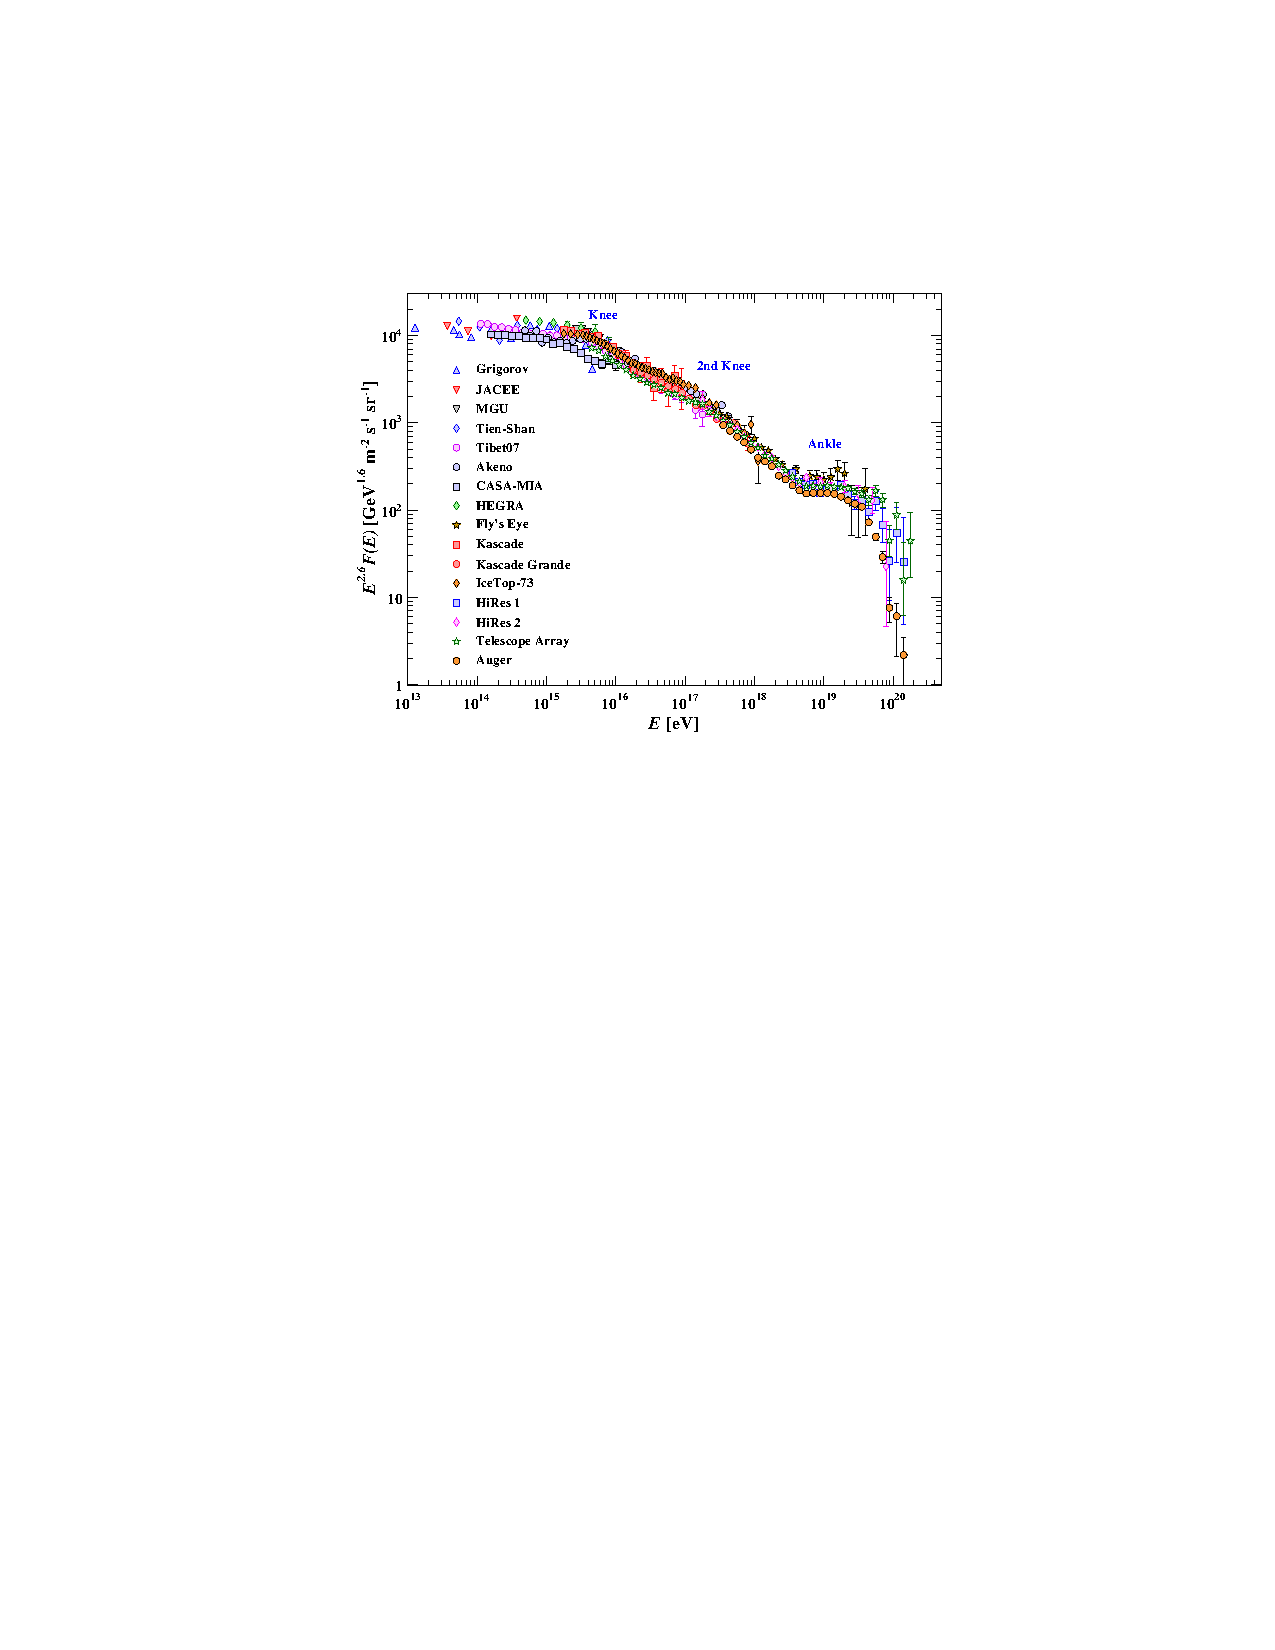
\includegraphics[width=0.6\textwidth]{./CosmicRays.pdf}
\caption{Observed energy distribution of cosmic rays (extra-galactic protons) from various experiments. The data are determined by measuring the energy of particles from air showers due cosmic rays hitting the upper atmosphere of Earth. From K.A. Olive et al. (Particle Data Group), Chin. Phys. C, 38, 010009 (2014) and 2015 update.}
\end{figure}


Compare your estimated cut off to this cosmic ray data. 
%The maximum energy that cosmic rays are recorded on this plot are at about (or just below) our calculated value of the GZK cutoff. 
Are there any cosmic rays observed with energies above the GZK cutoff?
%A more careful analysis (including the thermal nature of the CMB) actually shows that the GZK cutoff is about 5 × 1019 eV, and so there have been a few ultra-high energy cosmic rays observed that violate the GZK limit! It remains an open problem to explain the source of cosmic rays that violate the GZK cutoff.

%Let p_p and pγ be the initial proton and CMB photon four-vectors, and pp′ and pπ be the final proton and pion four-vectors.

%Rapidity. In experimental particle physics, it is often very useful to express the direction of motion of a particle in terms of its rapidity y. The rapidity is defined as
%y= 1logE+pz , (2.159) 2 E − pz
%for a particle with energy E and z-component of momentum pz. What makes rapidity so nice is its simple properties under Lorentz transformation. Perform a Lorentz boost of the energy and momentum along the zˆ axis with velocity β. How does the rapidity transform under this boost? You should be able to write the Lorentz-boosted rapidity as a simple function of the original rapidity.
%

\end{document}
